\PassOptionsToPackage{unicode=true}{hyperref} % options for packages loaded elsewhere
\PassOptionsToPackage{hyphens}{url}
%
\documentclass[english,jou,floatsintext]{apa7}
\usepackage{lmodern}
\usepackage{amssymb,amsmath}
\usepackage{ifxetex,ifluatex}
\usepackage{fixltx2e} % provides \textsubscript
\ifnum 0\ifxetex 1\fi\ifluatex 1\fi=0 % if pdftex
  \usepackage[T1]{fontenc}
  \usepackage[utf8]{inputenc}
  \usepackage{textcomp} % provides euro and other symbols
\else % if luatex or xelatex
  \usepackage{unicode-math}
  \defaultfontfeatures{Ligatures=TeX,Scale=MatchLowercase}
\fi
% use upquote if available, for straight quotes in verbatim environments
\IfFileExists{upquote.sty}{\usepackage{upquote}}{}
% use microtype if available
\IfFileExists{microtype.sty}{%
\usepackage[]{microtype}
\UseMicrotypeSet[protrusion]{basicmath} % disable protrusion for tt fonts
}{}
\IfFileExists{parskip.sty}{%
\usepackage{parskip}
}{% else
\setlength{\parindent}{0pt}
\setlength{\parskip}{6pt plus 2pt minus 1pt}
}
\usepackage{hyperref}
\hypersetup{
            pdftitle={Modelling disfluencies in copy-typing},
            pdfkeywords={Copy-task; keystroke modeling; autoregression; mixture models; Bayesian inference},
            pdfborder={0 0 0},
            breaklinks=true}
\urlstyle{same}  % don't use monospace font for urls
\usepackage{graphicx,grffile}
\makeatletter
\def\maxwidth{\ifdim\Gin@nat@width>\linewidth\linewidth\else\Gin@nat@width\fi}
\def\maxheight{\ifdim\Gin@nat@height>\textheight\textheight\else\Gin@nat@height\fi}
\makeatother
% Scale images if necessary, so that they will not overflow the page
% margins by default, and it is still possible to overwrite the defaults
% using explicit options in \includegraphics[width, height, ...]{}
\setkeys{Gin}{width=\maxwidth,height=\maxheight,keepaspectratio}
\setlength{\emergencystretch}{3em}  % prevent overfull lines
\providecommand{\tightlist}{%
  \setlength{\itemsep}{0pt}\setlength{\parskip}{0pt}}
\setcounter{secnumdepth}{0}

% set default figure placement to htbp
\makeatletter
\def\fps@figure{htbp}
\makeatother

% Manuscript styling
\usepackage{upgreek}
\captionsetup{font=singlespacing,justification=justified}

% Table formatting
\usepackage{longtable}
\usepackage{lscape}
% \usepackage[counterclockwise]{rotating}   % Landscape page setup for large tables
\usepackage{multirow}		% Table styling
\usepackage{tabularx}		% Control Column width
\usepackage[flushleft]{threeparttable}	% Allows for three part tables with a specified notes section
\usepackage{threeparttablex}            % Lets threeparttable work with longtable

% Create new environments so endfloat can handle them
% \newenvironment{ltable}
%   {\begin{landscape}\begin{center}\begin{threeparttable}}
%   {\end{threeparttable}\end{center}\end{landscape}}
\newenvironment{lltable}{\begin{landscape}\begin{center}\begin{ThreePartTable}}{\end{ThreePartTable}\end{center}\end{landscape}}

% Enables adjusting longtable caption width to table width
% Solution found at http://golatex.de/longtable-mit-caption-so-breit-wie-die-tabelle-t15767.html
\makeatletter
\newcommand\LastLTentrywidth{1em}
\newlength\longtablewidth
\setlength{\longtablewidth}{1in}
\newcommand{\getlongtablewidth}{\begingroup \ifcsname LT@\roman{LT@tables}\endcsname \global\longtablewidth=0pt \renewcommand{\LT@entry}[2]{\global\advance\longtablewidth by ##2\relax\gdef\LastLTentrywidth{##2}}\@nameuse{LT@\roman{LT@tables}} \fi \endgroup}

% \setlength{\parindent}{0.5in}
% \setlength{\parskip}{0pt plus 0pt minus 0pt}

% \usepackage{etoolbox}
\makeatletter
\patchcmd{\HyOrg@maketitle}
  {\section{\normalfont\normalsize\abstractname}}
  {\section*{\normalfont\normalsize\abstractname}}
  {}{\typeout{Failed to patch abstract.}}
\makeatother
\shorttitle{Modelling disfluencies in copy-typing}
\author{Jens Roeser\textsuperscript{1}, Sven De Maeyer\textsuperscript{2}, Mark Torrance\textsuperscript{1}, Luuk Van Waes\textsuperscript{3}, \& Mariëlle Leijten\textsuperscript{3}}
\affiliation{
\vspace{0.5cm}
\textsuperscript{1} Department of Psychology, Nottingham Trent University, United Kingdom\\\textsuperscript{2} Faculty of Social Sciences, University of Antwerp, Belgium\\\textsuperscript{3} Department of Management, University of Antwerp, Belgium}
\authornote{

Correspondence concerning this article should be addressed to Jens Roeser, 50 Shakespeare St, Nottingham NG1 4FQ. E-mail: jens.roeser@ntu.ac.uk}
\keywords{Copy-task; keystroke modeling; autoregression; mixture models; Bayesian inference}
\usepackage{dblfloatfix}


\usepackage{csquotes}
\usepackage{booktabs}
\usepackage{longtable}
\usepackage{array}
\usepackage{multirow}
\usepackage{float}
\usepackage{colortbl}
\usepackage{threeparttable}
\usepackage[normalem]{ulem}
\usepackage[utf8]{inputenc}
\ifnum 0\ifxetex 1\fi\ifluatex 1\fi=0 % if pdftex
  \usepackage[shorthands=off,main=english]{babel}
\else
  % load polyglossia as late as possible as it *could* call bidi if RTL lang (e.g. Hebrew or Arabic)
  \usepackage{polyglossia}
  \setmainlanguage[]{english}
\fi

\title{Modelling disfluencies in copy-typing}

\date{}

\abstract{
The analysis of keystroke data is typically performed on aggregates (mean, median). Aggregating data results in two basic problems. First, means are poor descriptives for non-normal distributed data. Second, using means artificially reduces information and adds bias to the estimates. In particular disfluencies affect these estimates. While many researchers use thresholds to define or trim data for certain purpuses, disfluencies are important indicators for increased cognitive demands and are ought to be addressed for statistical inference. We implemented a series of Bayesian models and tested these models on a random sample of 100 participants (age 18-25) from the Dutch copy-task corpus. Comparing the predictive performance of these models showed strong support for models that account for disfluencies as a mixture process allowing for a principle method of detecting disfluencies during keyboard typing.
}

\begin{document}
\maketitle

\hypertarget{introduction}{%
\section{Introduction}\label{introduction}}

Writing research has made extensive use of keystroke-logging to capture typing process data. In particular disfluencies (loosly defined as relatively long intervals between subsequent keystrokes) are interesting as these are indicators of processing demands (Chukharev-Hudilainen, Saricaoglu, Torrance, \& Feng, 2019) which may arise on various levels of mental representation (Olive, 2014); for example, when preplanning syntactic dependencies (Roeser, Torrance, \& Baguley, 2019), retrieving a lexical entry for a word or its spelling (Torrance, Rønneberg, Johansson, \& Uppstad, 2016). At present there is no principled way of determining which keystroke intervals constitute a process disfluency. In this paper we present a series of statistical models that aimed at capturing the typing process and in particular process disfluencies.

Keystroke logs provide very rich information about the typing process. To reduce the complexity of the data, researchers have often performed analysis on the means, medians, standard deviations (SD) etc. of inter-keystroke intervals (the duration between two consecutive keystrokes), number of pauses or pause durations, within-word keystroke intervals and many other variables (for an overview see Conijn, Roeser, \& van Zaanen, 2019). Conijn et al. (2019) suggested that different aggregates are sensitive to processing difficulty that arises on different levels of mental representation. However, using data aggregates comes with a number of problems. First, a feature such as pause duration or number of puases requires a definition what consitutes a pause. Researchs have often used a conventional but arbitrary threshold of 2 secs to define pauses (Alves \& Limpo, 2015; Chukharev-Khudilaynen, 2014; Connelly, Dockrell, Walter, \& Critten, 2012; Leijten \& Van Waes, 2013). Second, aggregating data artificially reduces the information in the data requires trimming criteria (Hoaglin \& Iglewicz, 1987) which remove certain data as outliers that might be valuable information about the writing processs. For example, data aggregation disregards timecourse variation and autocorrelation between consecutive keystrokes (Eltahir, Salami, Ismail, \& Lai, 2004). Third, parametric aggrgates such the mean and the SD function assume that, for the aggregated data point to be representative for the sample, keystroke intervals must come from a normal distribution. This is not the case as keystroke intervals are zero-bound and therefore right-skewed.\footnote{In fact, the minimum size of keystroke intervals is determined by the time it takes to plan and execute the motor programm.} Hence, aggregates are biased estimates of the typing process and therefore may lead to incorrect inference.

While the former problems are statistical problems they are interlinked with a conceptual issue. Statistical models make assumptions about the nature of the data generating process. For example, most standard statistical models assume that the data come from a single process that generates normal distributed data. We already addressed that keystroke data are not normal distributed. Another problem is that the underlying mental process that generates keystroke data involves cognitive processing on different levels mental representation. Process diffculty on any of these levels inhibits the acivation flow into lower levels of representation which then creates disfluencies (see Christiansen \& Chater, 2016; Olive, 2014). For example, copying a sequence of letters involves visual encoding of the sequence of letters, buffering n-bigrams in memory, identifying the correct key(s) on the keyboard, and programming and executing the relevant motor codes. Difficulty at any of these levels of processing will inhibit processing lower levels of activation which results in typing disfluencies. Further, the duration of the delay might, to some extent, depend on the level of activation that is causing the lag. Thresholds are insufficient to distinguish fluent from disfluent typing to force the typing process into a single normal distribution. Crutially important information about the mental process would be removed. Planning the next keystroke may in some cases be more demanding, in particular when planning on phrase boundaries or due to the retrieval of the lexical form of a low frequent word. Also, long values are more likely for struggling writers. For incorrectly produced keystroke intervals, durations may or may not change depending on whether the error was noticed by the participant or create a dysfluency for a subsequent keystroke interval. Importantly, long keystrokes are not necessarily outliers and pauses are a central part of the writing process.

\hypertarget{modelling-typing-process-data}{%
\section{Modelling typing process data}\label{modelling-typing-process-data}}

As a guiding principle, we aim to produce statistical models that are representative for the theoretical process that creates the data at hand. All models aim to model the typing process based on unaggregated data, i.e.~the lags between subseuqent keypresses; e.g.~c\(^{\wedge}\)a\(^{\wedge}\)t for typing the word \emph{cat}, where the caret \(^{\wedge}\) indicates the difference betwee the time for pressing \(<\)c\(>\) and \(<\)a\(>\). Further, our models aim to provide a systematic way of addressing process disfluencies rather than requiring data removal or pausing thresholds. For example when the time for pressing \(<\)a\(>\) after \(<\)c\(>\) is unusually large, our models should make notice of this disfluency.

We implement statistical models that aim to capture these keystroke interval data. Statistcal models allow us to characterise an underlying data generating process using parameters. For example if we assume that data com from a normal distribution, we can charactersie this distribution with a value \(\mu\) that indicates the centre of the distribution and a scale \(\sigma^2\) (i.e.~the variance); this can be expressed as \(y \sim Normal(\mu, \sigma^2)\). We will assume thoughout that the inter-keystroke interval (IKI) data can be characterised with a log-normal distribution, because IKIs are zero-bound and therefore right-skewed. Linear mixed effects models (LMM), as in equation \ref{eq:lmm}, are extensions of this logic which has been used widely for modelling keystroke data (Quené \& Van den Bergh, 2004; Van Waes, Leijten, \& Quinlan, 2010; Van Waes, Leijten, Roeser, Olive, \& Grabowski, 2020). Crutially, the parameters of interest can be estimated while accounting for variance that is unknown and random. For example, some participants are faster typists than others. The variance associated with the \(i\)s participant, expressed as \(u_i\), can be assumed to be normal distributed around 0 with a between participants variance \(\sigma_u^2\) with \(i = 1, \dots, I\), where \(I\) is the number of participants. After addressing individual typing-speed, the process that generates IKIs can be described by a mean \(\mu\) and an error variance \(\sigma_e^2\). For model fit purposes, the mean \(\mu\) was estimated using a non-centred parametrisation with weakly informative priors (Lambert, 2018). For the error variance we used a standard non-informative half-Cauchy prior (Gelman et al., 2014) as the variance must be larger than zero. Generally, we use weakly informative priors to aid model convergence. These priors help to reduce the parameter space to relatively plausible calues. All models presented below share these properties. The following models differ as to how (1) timecourse differences and (2) disfluencies are addressed by these models.

A standard approach to model the variation between individual keystroke pairs (i.e.~bigrams) is to assume that each bigram \(j\) with \(j = 1, \dots, J\), where \(I\) is the total number of bigrams, is independent of the other bigrams and associated with a unknown variance \(w_j\) that is distributed around 0 with a between bigram variance \(\sigma_w^2\) (see Van Waes, Leijten, Pauwaert, \& Van Horenbeeck, 2019).

\[
\tag{1}
\begin{aligned}
y_{ij} \sim LogNormal(\mu + u_i + w_j, \sigma_e^2)\\
\text{where}\\
\mu = \mu_{\alpha} + \mu_{\sigma} * \mu_{\eta}\\
\mu_{\alpha} \sim Normal(5,4)\\
\mu_{\sigma} \sim Normal(0,10)\\
\mu_{\eta} \sim Normal(0,1)\\
u_i \sim Normal(0, \sigma_u^2)\\
w_j \sim Normal(0, \sigma_w^2)\\
\sigma_u, \sigma_w \sim Normal(0,2.5)\\
\sigma_e \sim Cauchy(0,2.5)\\
\text{constraint: }\mu_{\sigma}, \sigma_u, \sigma_w, \sigma_e >0 
\end{aligned}
\label{eq:lmm}
\]

Further, we can extent this model by assuming that larger variations in typing differences for bigrams depend on the typing speed of each participant. For example, fast participants might show less variation between bigrams that slow participants. This assumption can be modelled by including by-participant slope adjustments for bigrams by introducing a variance-covariance matrix \(\Sigma_u\); LKJ prior with \(\nu=2.0\) (Lewandowski, Kurowicka, \& Joe, 2009).

\hypertarget{typing-as-autoregressive-process}{%
\subsection{Typing as autoregressive process}\label{typing-as-autoregressive-process}}

The standard analysis can model variation that is associated with particular bigrams but does allow us to address disfluencies in the typing process beyond assuming they are subject to random statistical noise. Further, the standard analysis assumes that subsequent keystrokes are independent and thus exchangable. If we assume that subsequent keystrokes are autocorrelated (Eltahir et al., 2004), a disfluency can be characterised as a slowdown relative to the previous keystroke interval. In other words, we can predict IKIs with the previous keystroke interval. This feature is at the heart of autoregressive models. These models capture the autocorrelation between subsequent keystrokes by introducing a parameter \(\phi\) that predicts an IKI \(y_j\) on the basis of the IKI preceding it \(y_{j-1}\); see equation \ref{eq:ark}. \(\phi_i\) was estimated separately for each participant with a pooled mean \(\phi\) and error variance \(\eta^2\). Note, to allow comparisons between this and all other models we had exclude the first bigram for each participant, i.e. \(y_{ij+1}\).

\[
\tag{2}
\begin{aligned}
y_{ij} \sim LogNormal(\mu + \phi_i*log(y_{ij-1}) + u_i, \sigma_e^2)\\
\text{where}\\
\mu = \mu_{\alpha} + \mu_{\sigma} * \mu_{\eta}\\
\phi_i \sim Normal(\phi, \eta^2)\\
\mu_{\alpha} \sim Normal(5,4)\\
\mu_{\sigma} \sim Normal(0,10)\\
\mu_{\eta}, \phi \sim Normal(0, 1)\\
\eta \sim Cauchy(0, 1)\\
u_i \sim Normal(0, \sigma_u^2)\\
\sigma_u \sim Normal(0,2.5)\\
\sigma_e \sim Cauchy(0,2.5)\\
\text{constraint: }\mu_{\sigma}, \sigma_u, \sigma_e, \eta >0 
\end{aligned}
\label{eq:ark}
\]

\hypertarget{typing-as-autoregressive-finite-mixture-process}{%
\subsection{Typing as (autoregressive) finite mixture process}\label{typing-as-autoregressive-finite-mixture-process}}

Writing data are generally speaking a combination of fluent typing and typing disfluencies. While disfluencies can be subject to processing on various levels of mental representations they will always be expressed as longer keystroke intervals. To capture this mixture of fluent and disfluent typing, we implemented a finite mixture model. Mixture models assume that data come from a combination of distributions. For the present purpose we constrain the model to be finite. In other words, we fixed the number of underlying distributions to two, namely, 2 log-Gaussian (normal) distributions of which on represents fluent tying (shorter keystroke intervals) and the other process disfluencies (longer keystroke intervals). This model can be summarised as in equation \ref{eq:mog}, following Vasishth, Chopin, Ryder, and Nicenboim (2017). Both distributions have the same mean \(\mu\) but for the first the parameter \(\delta\) that was constrainted to be positive was added. The mixing proportion \(\theta_i\), then, captures the probability of a data point to be part of either distribution (fluent or disfluent typing) for each participant \(i\) which a mean \(\theta\) and variance \(\tau^2\). The mixing proportion \(\theta_i\) was transformed to range from 0 to 1 (inverse logit) where a value of 0 would indicate fluent typing and 1 indicates disfluency. As longer latencies are known to be associated with a larger variances for both response-time data in particular (Wagenmakers \& Brown, 2007) and human motor bahaviour in general (Schöner, 2002; Wing \& Kristofferson, 1973), the variance \(\sigma_{e'}^2\) associated with the distribution of typing disfluencies was constrained to be larger than the variance for normal typing \(\sigma_e^2\) .

\[
\tag{3}
\begin{aligned}
    y_{ij} \sim \theta_i \cdot LogNormal(\mu + \delta + u_i + w_j, \sigma_{e'}^2) +\\
        (1 - \theta_i) \cdot LogNormal(\mu + u_i + w_j, \sigma_{e}^2)\\
        \text{where}\\
        \theta_i = InvLogit(\theta_i)\\
        \mu = \mu_{\alpha} + \mu_{\sigma} * \mu_{\eta}\\
        \sigma_{e'} = \sigma + \sigma_{\text{diff}}\\
        \sigma_{e} = \sigma - \sigma_{\text{diff}}\\
        \theta_i \sim Normal(\theta,\tau^2)\\
    \mu_{\alpha} \sim Normal(5,4)\\
    \mu_{\sigma} \sim Normal(0,10)\\
        \theta, \delta, \mu_{\eta}, \sigma_{\text{diff}} \sim Normal(0,1)\\
        \tau \sim Cauchy(0,1)\\
        u_i \sim Normal(0, \sigma_u^2)\\
    w_j \sim Normal(0, \sigma_w^2)\\
    \sigma_u, \sigma_w \sim Normal(0,2.5)\\
        \sigma \sim Cauchy(0,2.5)\\
        \text{constraint: } \mu_{\sigma}, \sigma_u, \sigma_w, \delta, \tau, \sigma, \sigma_{\text{diff}}, \sigma_{e'}, \sigma_{e} > 0
\end{aligned}   
\label{eq:mog}
\]

Note that the former model implies that subsequent keystroke intervals are independent. This might be the case for disfluencies but fluent typing might involve autocorrelations. Therefore, we implemented another mixture model but replaced the bigram intercepts \(w_j\) in the previous model with an autoregressor \(\phi_i*y_{ij-1}\) in the distribution that represents fluent typing, as in equation \ref{eq:ark}, but included random bigram intercepts for the distribution of disfluent typing intervals.

\hypertarget{method}{%
\section{Method}\label{method}}

We evaluate our models using data from a subset of the Dutch copy-task corpus (Leijten \& Van Waes, 2013; Van Waes et al., 2019; Van Waes et al., 2020). The copy-task corpus consists of keystroke data collected in Inputlog, a Javascript-based web application, available on \url{www.inputlog.net}. In this analysis we focus on the consonant task because it is a demanding but short task that allows us to measure typing skills in a non-linguistic environment (Grabowski, Weinzierl, \& Schmitt, 2010). The consonant task is relatively short but complex in the sense that participants have to look at the target string repeatedly to copy it accurately. In other words, for this task we need to be able to disentagle fluent and disfluent latencies. Participants saw and copy-typed four blocks of six consonant sequences \enquote{tjxgfl pgkfkq dtdrgt npwdvf} that do not occur adjacently in Dutch. The dependent variable are the inter-keystroke intervals (IKI) between two consecutive consonants (key presses). Spaces were excluded from the data. From this corpus we took a random sample of 100 participants (78 female, 22 male) in the age range between 18 and 25 years (median age = 22 years). We used decided this age range to keep the sample relatively homogeneous.

\hypertarget{results}{%
\section{Results}\label{results}}

\hypertarget{data-overview}{%
\subsection{Data overview}\label{data-overview}}

The data are visualized in Figure \ref{fig:descriptives}. The figure shows the variations of IKIs throughout the copy-typing process. Each grey line represents one participant and the coloured lines shown different measures of central tendency. The central tendency descriptives represent different properties of the distribution as can be seen in the density plot in the right margin. The mean is sensitive to larger IKIs and is therefore in the centre of the distribution while the mode and the median are closer to the most frequent value. All central tendencies vary depending on the position of the bigram in the string. The up-and-down pattern in the data suggests that IKIs are sensitive to the position of a bigram in a chunk rather than bigram identity or the position of the bigram in the entire sequence.

\begin{figure}[!ht]

{\centering 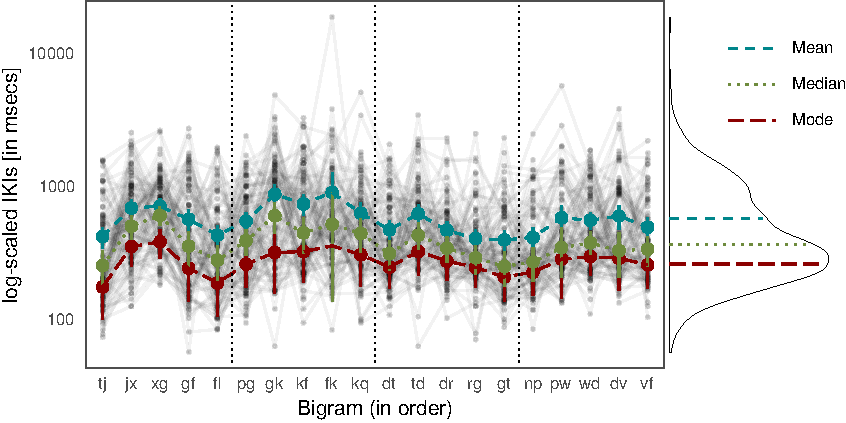
\includegraphics{frontline_files/figure-latex/descriptives-1} 

}

\caption{IKI data by participant over bigrams position shown in order. Shown are the raw data, each line representing one participant, and different measures of central tendency (with 2$\times$standard error [SE]). Vertical lines indicate the position of SPACES. The density distribution of IKI data is shown in the right margin.}\label{fig:descriptives}
\end{figure}

\hypertarget{model-comparisons}{%
\subsection{Model comparisons}\label{model-comparisons}}

All models were implemented as Bayesian models (see e.g. Gelman et al., 2014; Lambert, 2018; McElreath, 2016) in the probabilistic programming language Stan (Carpenter et al., 2016; Hoffman \& Gelman, 2014; Stan Development Team, 2015a, 2015b). \textit{R} and \textit{Stan} code are available on \href{https://github.com/jensroes/Frontline}{GitHub} for reproducibility. Models were fitted with weakly regulating priors and run with 30,000 iterations (15,000 warm-up) on 3 Markov chain Monte Carlo chains. Convergence was tested via the Rubin-Gelman statistic (Gelman \& Rubin, 1992), traceplots and cross-validation (Vehtari, Gelman, \& Gabry, 2015, 2017).

The predictive performance of the models was established using leave-one-out cross-validation which penalizes models with more parameters (see Farrell \& Lewandowsky, 2018; Lambert, 2018; Lee \& Wagenmakers, 2014; McElreath, 2016). The out-of-sample predictive performance was determined via Pareto smoothed importance-sampling (Vehtari et al., 2015, 2017) and estimated as sum of the expected log predictive density (\(\widehat{elpd}\)). \(\widehat{elpd}\) was used to compare the predictive quality of our models. Model comparisons can be found in Table \ref{tab:modelcomparisons}. The best fitting model was revealed to be the mixture model M4 (see equation \ref{eq:mog}).

\begin{table*}[!ht]

\begin{center}
\begin{threeparttable}

\caption{\label{tab:modelcomparisons}Model comparisons $\Delta\widehat{elpd}$ expressed as expected log predictive density ($\widehat{elpd}$) with SE in parentheses. The bigrams column indicates how the models account for by-bigram variation. The top row shows the model with the highest predictive performance.}

\begin{tabular}{llrrl}
\toprule
Model & \multicolumn{1}{c}{Type} & \multicolumn{1}{c}{$\Delta\widehat{elpd}$} & \multicolumn{1}{c}{$\widehat{elpd}$} & \multicolumn{1}{c}{Bigrams}\\
\midrule
M4 & MoG & 0 (0) & -13857 (59) & Random intercepts\\
M5 & AR + MoG & -14 (14) & -13871 (57) & Autoregressor $\phi$ and random intercepts\\
M2 & LMM & -87 (24) & -13944 (53) & Random intercepts and slopes\\
M1 & LMM & -153 (18) & -14010 (54) & Random intercepts\\
M3 & AR & -223 (21) & -14080 (54) & Autoregressor $\phi$\\
\bottomrule
\addlinespace
\end{tabular}

\begin{tablenotes}[para]
\normalsize{\textit{Note.} LMM = linear mixed effects models; AR = Autoregressive model; MoG = Mixture of (log-)Gaussians}
\end{tablenotes}

\end{threeparttable}
\end{center}

\end{table*}

The second best performing model is the mixture model with the autoregressor \(phi\) for fluent typing. In other words, adding the autoregressor instead of random bigram intercepts for fluent typing did not improve the predictive performance of the model. In fact, the autoregressive model was found to be the model with the lowest predictive performance among the models tested. Modelling bigrams as random intercepts (with and without by-participant slope adjustements) was found to have a higher predictive performance compared to the autoregession model (Van Waes et al., 2010, 2020). Overall the best fit among the tested models was revealed by the mixture model with a distribution for fluent typing and a distribution for disfluencies while accounting for bigrams as random variance.

\hypertarget{model-evaluation}{%
\subsection{Model evaluation}\label{model-evaluation}}

The copy-typing process captured by the mixture model can be assessed using the posterior distributions of the parameter values. The process relevant model parameter values are illustrated in Figure \ref{fig:parameters}. Firstly, IKIs, excluding disfluencies, are shown by participant in Figure \ref{fig:parameters}A. The red line indicates the pooled overall parameter estimate for fluent typing \(\hat{\beta}\)=259 msecs centred around a 95\% PI of {[}235, 286{]}. For each participant the probability of disfluent typing is shown in Figure \ref{fig:parameters}B. The overall disfluency probability (in red) was \(\hat{\theta}\)=0.73 centred around 95\% PI{[}0.63, 0.83{]}. In other words, for the consonant task we observe 73\% disfluent typing, and hence 27\% fluent typing.

The y-axis in panel A and B are ordered by the average size of the respective values, thus the lines do not represent the same participants. In fact, Figure \ref{fig:parameters}C suggests that the inferred latency for fluent typing and the probability to exhibit dislfuences are independent. Shown are the parameter estimates for each participant and the overall pooled estimates. In other words, the frequency of process disfluencies does not depend on the average typing speed. Fast as well as slow copy-typists can show low and high disfluency probabilities. Finally, the slowdown for disfluent typing is shown in Figure \ref{fig:parameters}D. Disfluent typing in the consonent task is \(\hat{\delta}\)=297 msecs (95\% PI{[}251, 347{]}) slower than fluent typing.\footnote{The size of the disfluency \(\delta\) could in principle vary by participant. For example, for faster participants might show larger disfluencies and slower participants might show smaller disfluencies. We addressed this possibility by allowing the disfluency parameter \(\delta\) to vary for each participant. This model reavealed a negligible gain over model M4 (\(\Delta\widehat{elpd}=\)-3, SE=2).} Overall, there is a large probability of dysfluent typing in the consonant task. This makes it crutial to distinguish between keystroke intervals that represent fluent and disfluent typing. Mixture models can provide accurate estimates for fluent typing by accounting disfluencies in a principled matter; i.e.~be modelling fluent and disfluent typing as a mixture process.

\begin{figure}[!ht]

{\centering 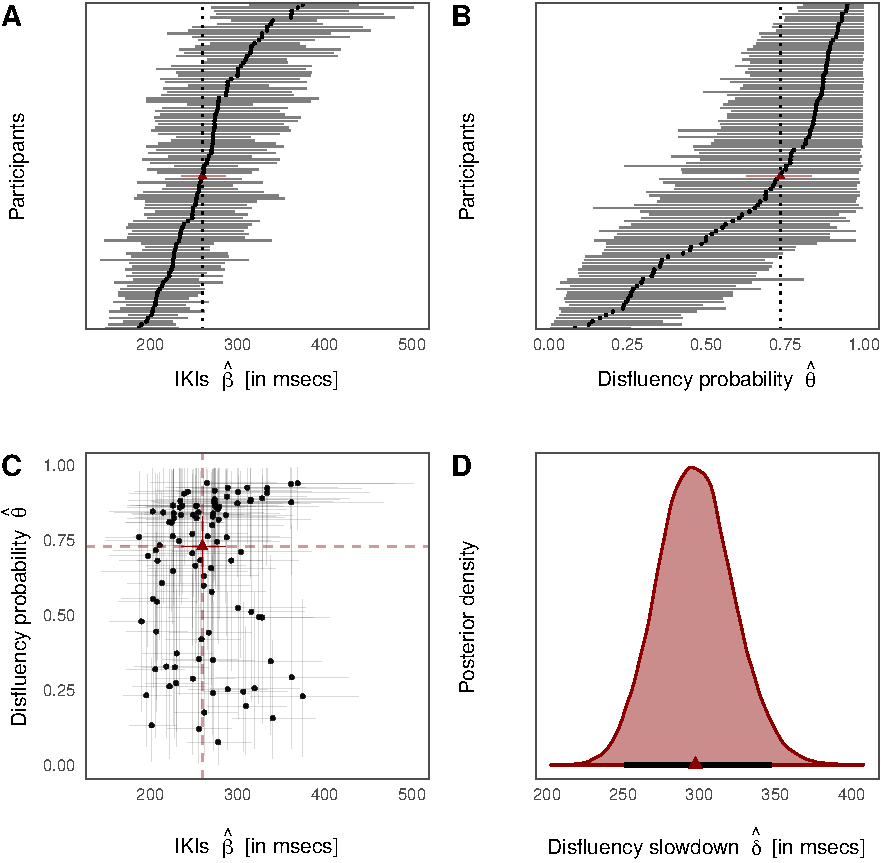
\includegraphics{frontline_files/figure-latex/parameters-1} 

}

\caption{Posterior parameter values of the mixture model. Panel A shows by-participant IKIs and overall IKI value for fluent typing in red. Panel B shows by-participant disfluency probability (overall parameter value $\theta$ in red). Panel C shows fluent IKIs plotted against disfluency probability (red triangle indicates overall parameter value). Panel D shows the posterior distribution of the disfluency slowdown. All error bars are 95\% probability intervals.}\label{fig:parameters}
\end{figure}

\hypertarget{discussion}{%
\section{Discussion}\label{discussion}}

Our aim was provide a statistical model of inter-keystroke intervals that addresses process disfluencies in a principled manner. We compared series of Bayesian models addressing this aim. Model comparisons showed that, among our models, process disfluencies can be captured best as a mixture process. This model captures disfluencies in the typing process by assuming that typing data come from a combination of two distributions, representing fluent and disfluent typing, of which each has a latent probability. This model allows us to extract reliable typing-interval estimates for fluent typing while accounting for process difluencies in a principled manner.

This model provides a) overall and by-participant keystroke intervals for fluent tpying, b) overall and by-participant disfluency probabilities, and c) an parameter estimate that captures the overall slowdown for disfluent trials. These parameter estimates are relevant on two levels. First, they allows us to characterise the writing task at hand. For example, we obseve that copy-typing non-lexical strings of consonants is ridden with disfluencies. Second, by-participant parameter estimates all us to extract typing characteristics for individual typists. In particular, we extracted each participants fluent typing speed and the probability of disfluencies exhibited by each participant. Taken both, overall and individual parameter estimates together, we can determine whether an individual typist was a fast / slow typist or had unusually high / low probability to exhibit disfluencies.

The central advantage of using mixture models to account for typing disfluencies is that we can by-pass the use of treshold values to define disfluencies. From the raw data it is not possible to know which data are disfluencies a priori. Using threshold values merely ignores that some participants are generally lower typists and some tasks are easier or more difficult. Mixture models allow us to capture disfluencies as a latent process in a principled way. This is important because the mixture model presented in this paper takes into account that a disfluency is relative to an individuals tpying speed. Therefore, this would allow to test predictions about typing disfluencies in certain population such as very young or old typists, language learners or individuals with genuine typing difficulty after account for individual differences in typing speed. Further while we used a relatively difficult copy-task to test our models, other writing tasks are bound to lead to other disfluency estimates. In fact, the presented model can be used to test hypothesis about psychological factors that might lead to varying proportions of disfluencies, and thefore changes in cognitive demands, in the writing process. As an avenue for future research, mixture models as presented in this paper can be used for different types of writing tasks and particular populations.

Writing involves processing on various cognitive levels, from generating an idea, retriving lexical entries to the encoding of spelling. As activation between these levels cascades from higher to lower levels of representation, a delay at any of these levels will cause disfluencies. In other words, disfluencies are not just an interesting but a central part of the writing process. Mixture models allows us to address the assumed combination of processes that underlies writing by mapping these of a combination of distributions. Using a combination of two distributions is merely reducing this combination into normal, fluent, typing and typing that involves processing delays on higher levels (i.e.~disfluencies). If one assumes that the size of the disfluency depends on the inhibited upstream process, one may implement this as an additional mixture component (see e.g. Baaijen, Galbraith, \& Glopper, 2012) for address different types of disfluencies (Wengelin, 2001).

\hypertarget{references}{%
\section{References}\label{references}}

\begingroup
\setlength{\parindent}{-0.5in}
\setlength{\leftskip}{0.5in}

\hypertarget{ref}{}

\endgroup

\hypertarget{refs}{}
\leavevmode\hypertarget{ref-alves2015progress}{}%
Alves, R. A., \& Limpo, T. (2015). Progress in written language bursts, pauses, transcription, and written composition across schooling. \emph{Scientific Studies of Reading}, \emph{19}(5), 374--391.

\leavevmode\hypertarget{ref-baaijen2012keystroke}{}%
Baaijen, V. M., Galbraith, D., \& Glopper, K. de. (2012). Keystroke analysis: Reflections on procedures and measures. \emph{Written Communication}, \emph{29}(3), 246--277.

\leavevmode\hypertarget{ref-carpenter2016stan}{}%
Carpenter, B., Gelman, A., Hoffman, M. D., Lee, D., Goodrich, B., Betancourt, M., \ldots{} Riddell, A. (2016). Stan: A probabilistic programming language. \emph{Journal of Statistical Software}, \emph{20}.

\leavevmode\hypertarget{ref-christiansen2016now}{}%
Christiansen, M. H., \& Chater, N. (2016). The now-or-never bottleneck: A fundamental constraint on language. \emph{Behavioral and Brain Sciences}, \emph{39}, 1--72. \href{https://doi.org/\%20http://dx.doi.org/10.1017/S0140525X1500031X}{https://doi.org/ http://dx.doi.org/10.1017/S0140525X1500031X}

\leavevmode\hypertarget{ref-chukharev2019combined}{}%
Chukharev-Hudilainen, E., Saricaoglu, A., Torrance, M., \& Feng, H.-H. (2019). Combined deployable keystroke logging and eyetracking for investigating L2 writing fluency. \emph{Studies in Second Language Acquisition}, \emph{41}(3), 583--604.

\leavevmode\hypertarget{ref-chukharev2014pauses}{}%
Chukharev-Khudilaynen, E. (2014). Pauses in spontaneous written communication: A keystroke logging study. \emph{Journal of Writing Research}, \emph{6}(1), 61--84.

\leavevmode\hypertarget{ref-conijn2019understanding}{}%
Conijn, R., Roeser, J., \& van Zaanen, M. (2019). Understanding the keystroke log: The effect of writing task on keystroke features. \emph{Reading and Writing}, \emph{32}(9), 2353--2374.

\leavevmode\hypertarget{ref-connelly2012predicting}{}%
Connelly, V., Dockrell, J. E., Walter, K., \& Critten, S. (2012). Predicting the quality of composition and written language bursts from oral language, spelling, and handwriting skills in children with and without specific language impairment. \emph{Written Communication}, \emph{29}(3), 278--302.

\leavevmode\hypertarget{ref-eltahir2004dynamic}{}%
Eltahir, W. E., Salami, M., Ismail, A. F., \& Lai, W. (2004). Dynamic keystroke analysis using AR model. In \emph{IEEE international conference on industrial technology} (Vol. 3, pp. 1555--1560). IEEE.

\leavevmode\hypertarget{ref-farrell2018computational}{}%
Farrell, S., \& Lewandowsky, S. (2018). \emph{Computational modeling of cognition and behavior}. Cambridge University Press.

\leavevmode\hypertarget{ref-gelman2014}{}%
Gelman, A., Carlin, J. B., Stern, H. S., Dunson, D. B., Vehtari, A., \& Rubin, D. B. (2014). \emph{Bayesian data analysis} (3rd ed.). Chapman; Hall/CRC.

\leavevmode\hypertarget{ref-gelman1992}{}%
Gelman, A., \& Rubin, D. B. (1992). Inference from iterative simulation using multiple sequences. \emph{Statistical Science}, \emph{7}(4), 457--472.

\leavevmode\hypertarget{ref-grabowski2010second}{}%
Grabowski, J., Weinzierl, C., \& Schmitt, M. (2010). Second and fourth graders' copying ability: From graphical to linguistic processing. \emph{Journal of Research in Reading}, \emph{33}(1), 39--53.

\leavevmode\hypertarget{ref-hoaglin1987fine}{}%
Hoaglin, D. C., \& Iglewicz, B. (1987). Fine-tuning some resistant rules for outlier labeling. \emph{Journal of the American Statistical Association}, \emph{82}(400), 1147--1149.

\leavevmode\hypertarget{ref-hoffman2014no}{}%
Hoffman, M. D., \& Gelman, A. (2014). The No-U-Turn sampler: Adaptively setting path lengths in Hamiltonian Monte Carlo. \emph{Journal of Machine Learning Research}, \emph{15}(1), 1593--1623.

\leavevmode\hypertarget{ref-lambert2018student}{}%
Lambert, B. (2018). \emph{A student's guide to Bayesian statistics}. Sage.

\leavevmode\hypertarget{ref-lee2014bayesian}{}%
Lee, M. D., \& Wagenmakers, E.-J. (2014). \emph{Bayesian cognitive modeling: A practical course}. Cambridge University Press.

\leavevmode\hypertarget{ref-leijten2013keystroke}{}%
Leijten, M., \& Van Waes, L. (2013). Keystroke logging in writing research: Using Inputlog to analyze and visualize writing processes. \emph{Written Communication}, \emph{30}(3), 358--392.

\leavevmode\hypertarget{ref-lewandowski2009generating}{}%
Lewandowski, D., Kurowicka, D., \& Joe, H. (2009). Generating random correlation matrices based on vines and extended onion method. \emph{Journal of Multivariate Analysis}, \emph{100}(9), 1989--2001.

\leavevmode\hypertarget{ref-mcelreath2016statistical}{}%
McElreath, R. (2016). \emph{Statistical rethinking: A bayesian course with examples in R and Stan}. CRC Press.

\leavevmode\hypertarget{ref-olive2014toward}{}%
Olive, T. (2014). Toward a parallel and cascading model of the writing system: A review of research on writing processes coordination. \emph{Journal of Writing Research}, \emph{6}(2), 173--194.

\leavevmode\hypertarget{ref-quene2004multi}{}%
Quené, H., \& Van den Bergh, H. (2004). On multi-level modeling of data from repeated measures designs: A tutorial. \emph{Speech Communication}, \emph{43}(1-2), 103--121.

\leavevmode\hypertarget{ref-roeser2019advance}{}%
Roeser, J., Torrance, M., \& Baguley, T. (2019). Advance planning in written and spoken sentence production. \emph{Journal of Experimental Psychology: Learning, Memory, and Cognition}, \emph{45}(11), 1983--2009.

\leavevmode\hypertarget{ref-schoner2002timing}{}%
Schöner, G. (2002). Timing, clocks, and dynamical systems. \emph{Brain and Cognition}, \emph{48}(1), 31--51.

\leavevmode\hypertarget{ref-rstan}{}%
Stan Development Team. (2015a). Stan: A C++ library for probability and sampling. \url{http://mc-stan.org/}.

\leavevmode\hypertarget{ref-rstan2}{}%
Stan Development Team. (2015b). Stan modeling language user's guide and reference manual. \url{http://mc-stan.org/}.

\leavevmode\hypertarget{ref-torrance2016adolescent}{}%
Torrance, M., Rønneberg, V., Johansson, C., \& Uppstad, P. H. (2016). Adolescent weak decoders writing in a shallow orthography: Process and product. \emph{Scientific Studies of Reading}, \emph{20}(5), 375--388.

\leavevmode\hypertarget{ref-van2019multilingual}{}%
Van Waes, L., Leijten, M., Pauwaert, T., \& Van Horenbeeck, E. (2019). A multilingual copy task: Measuring typing and motor skills in writing with inputlog. \emph{Journal of Open Research Software}, \emph{7}(30), 1--8.

\leavevmode\hypertarget{ref-van2010reading}{}%
Van Waes, L., Leijten, M., \& Quinlan, T. (2010). Reading during sentence composing and error correction: A multilevel analysis of the influences of task complexity. \emph{Reading and Writing}, \emph{23}(7), 803--834. \url{https://doi.org/10.1007/s11145-009-9190-x}

\leavevmode\hypertarget{ref-waes2019}{}%
Van Waes, L., Leijten, M., Roeser, J., Olive, T., \& Grabowski, J. (2020). Designing a copy task to measure typing and motor skills in writing research. \emph{Journal of Writing Research}.

\leavevmode\hypertarget{ref-vasishth2017}{}%
Vasishth, S., Chopin, N., Ryder, R., \& Nicenboim, B. (2017). Modelling dependency completion in sentence comprehension as a Bayesian hierarchical mixture process: A case study involving Chinese relative clauses. \emph{ArXiv E-Prints}.

\leavevmode\hypertarget{ref-vehtari2015pareto}{}%
Vehtari, A., Gelman, A., \& Gabry, J. (2015). Pareto smoothed importance sampling. \emph{arXiv Preprint arXiv:1507.02646}.

\leavevmode\hypertarget{ref-vehtari2017practical}{}%
Vehtari, A., Gelman, A., \& Gabry, J. (2017). Practical bayesian model evaluation using leave-one-out cross-validation and WAIC. \emph{Statistics and Computing}, \emph{27}(5), 1413--1432.

\leavevmode\hypertarget{ref-wagenmakers2007linear}{}%
Wagenmakers, E.-J., \& Brown, S. (2007). On the linear relation between the mean and the standard deviation of a response time distribution. \emph{Psychological Review}, \emph{114}(3), 830--841. \url{https://doi.org/10.1037/0033-295X.114.3.830}

\leavevmode\hypertarget{ref-wengelin2001disfluencies}{}%
Wengelin, Å. (2001). Disfluencies in writing -- Are they like in speaking? In \emph{ISCA tutorial and research workshop (ITRW) on disfluency in spontaneous speech}.

\leavevmode\hypertarget{ref-wing1973response}{}%
Wing, A. M., \& Kristofferson, A. B. (1973). Response delays and the timing of discrete motor responses. \emph{Perception \& Psychophysics}, \emph{14}(1), 5--12.

\end{document}
